\documentclass[10pt,a4paper]{article}
\usepackage[margin=19mm]{geometry}
\usepackage[T1]{fontenc}
\usepackage{lmodern,amsmath,graphicx,xcolor,float}
\usepackage{microtype}
\usepackage[colorlinks=true,urlcolor=blue!55!black,linkcolor=blue!55!black]{hyperref}
\usepackage[font=small,labelfont=bf]{caption}
\setlength{\parindent}{0pt}
\setlength{\parskip}{5pt}
\graphicspath{{figures/}}
\newcommand{\src}[2]{\href{#2}{[S#1]}}
\begin{document}
\begin{center}
{\Large\bfseries Electrical power delivery for endothermic reactors}\par\vspace{4pt}
{\large Available systems and reactor matching}\par\vspace{3pt}
Evidence snapshot: 8 September 2026
\end{center}

\section{Available power systems}
Electrification can intensify endothermic processing when it improves where and how energy enters the reacting material. The initial objective is a power architecture capable of at least 100~MW aggregate output. Published industrial data make low-kilohertz converters a credible starting point, but do not establish an optimum frequency or a universal decline in performance with increasing frequency.

Figure~\ref{fig:evidence} compares selected published offerings and installations. SMS lists 0.4--4~MW LLC converters at 1--10~kHz [S2]; Meltech quotes approximately 98\% operating efficiency for its 0.2--10~kHz family [S3]. These are separate sources: the data do not establish 98\% efficiency for the 4~MW SMS unit. Higher-frequency examples include CEIA's family claim of $>96\%$ at 100--400~kHz [S5,S6], and microwave generators quoting approximately 80--85\% [S9,S10]. Efficiency definitions and operating conditions differ, so these points should not be fitted as a common efficiency curve.

\begin{figure}[ht]
\centering
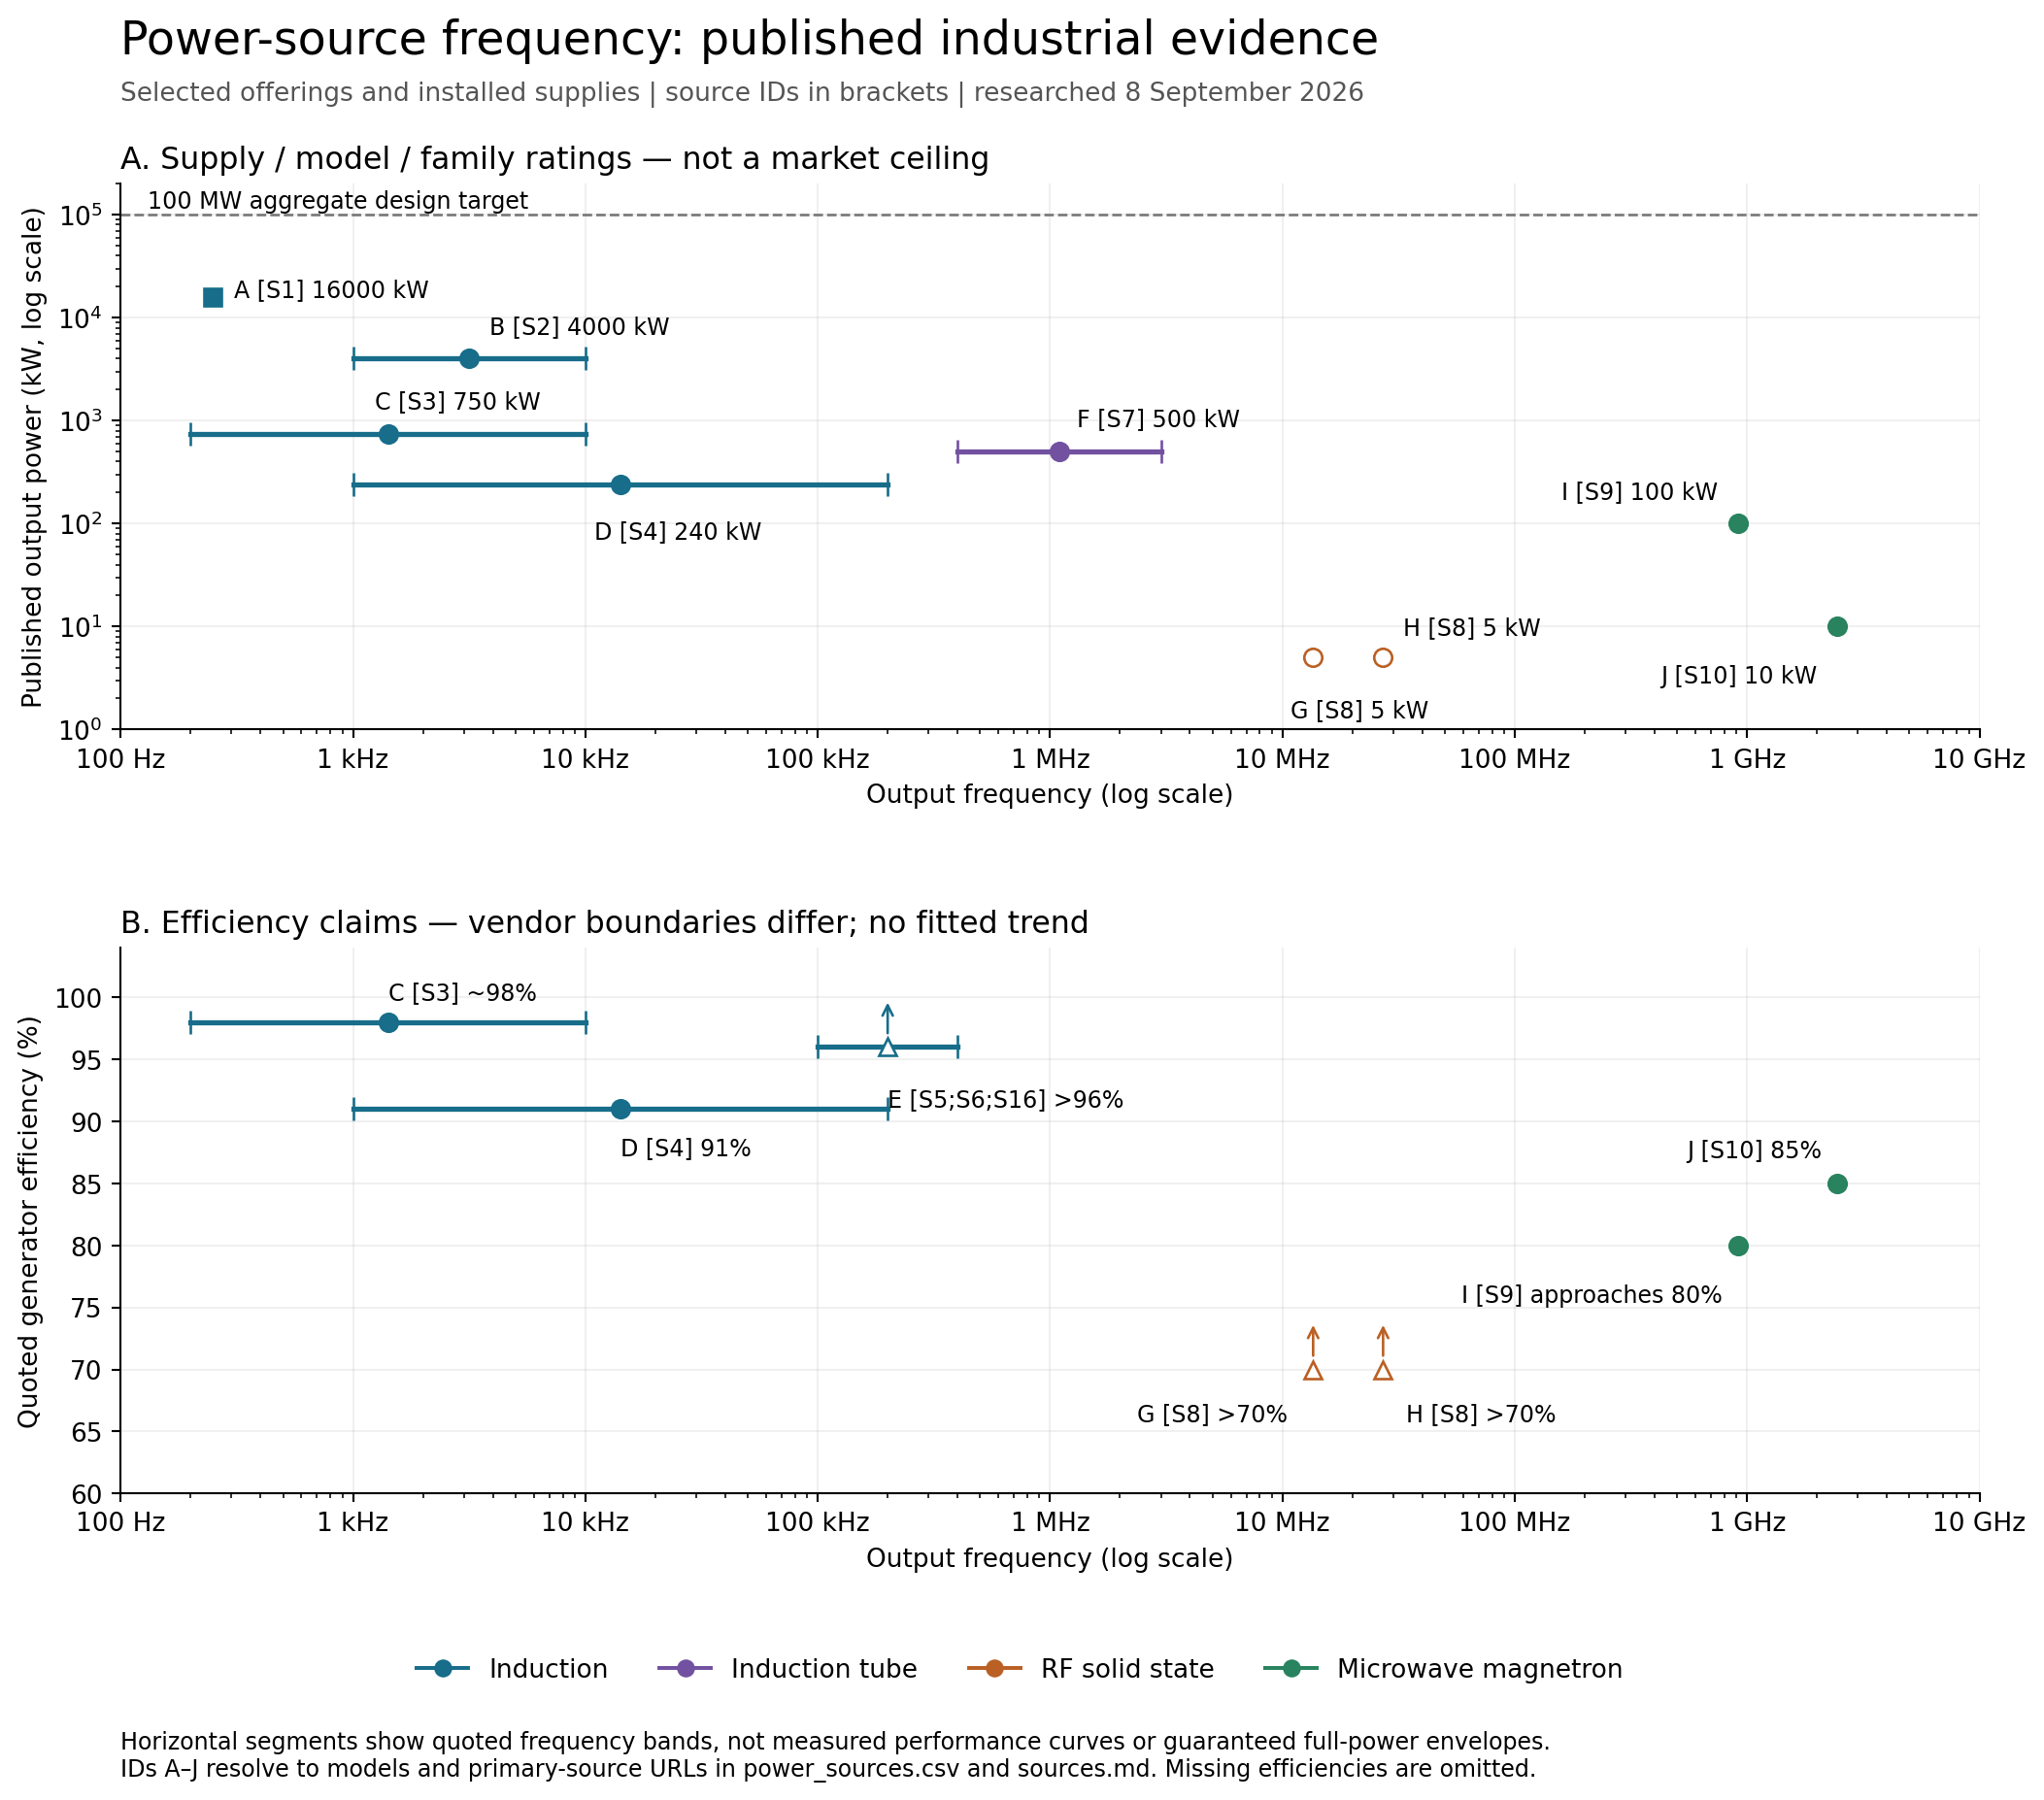
\includegraphics[width=\linewidth,height=.60\textheight,keepaspectratio]{frequency_evidence.png}
\caption{Published frequency, output-power and efficiency evidence. Source identifiers resolve to clickable references on the final page. Horizontal segments are quoted bands, not measured curves or guaranteed simultaneous operating envelopes. CEIA's 50~kW rating is input power and is omitted from the output-power panel [S16].}
\label{fig:evidence}
\end{figure}

\clearpage
\textbf{Scale and pulsed operation.} ABP reports a 16~MW supply at 250~Hz and a separate installation with three 42~MW supplies, totalling 126~MW [S1]. The latter's exact frequency is unavailable and is not assigned a frequency coordinate. Commercially listed specialist klystrons also reach 1.2~MW continuous output around 0.5--1.25~GHz, with 63\% tube efficiency [S13]. These require upstream supplies and auxiliaries: high-frequency megawatt output exists, but its efficiency and integration requirements differ from industrial converters.

\begin{figure}[ht]
\centering
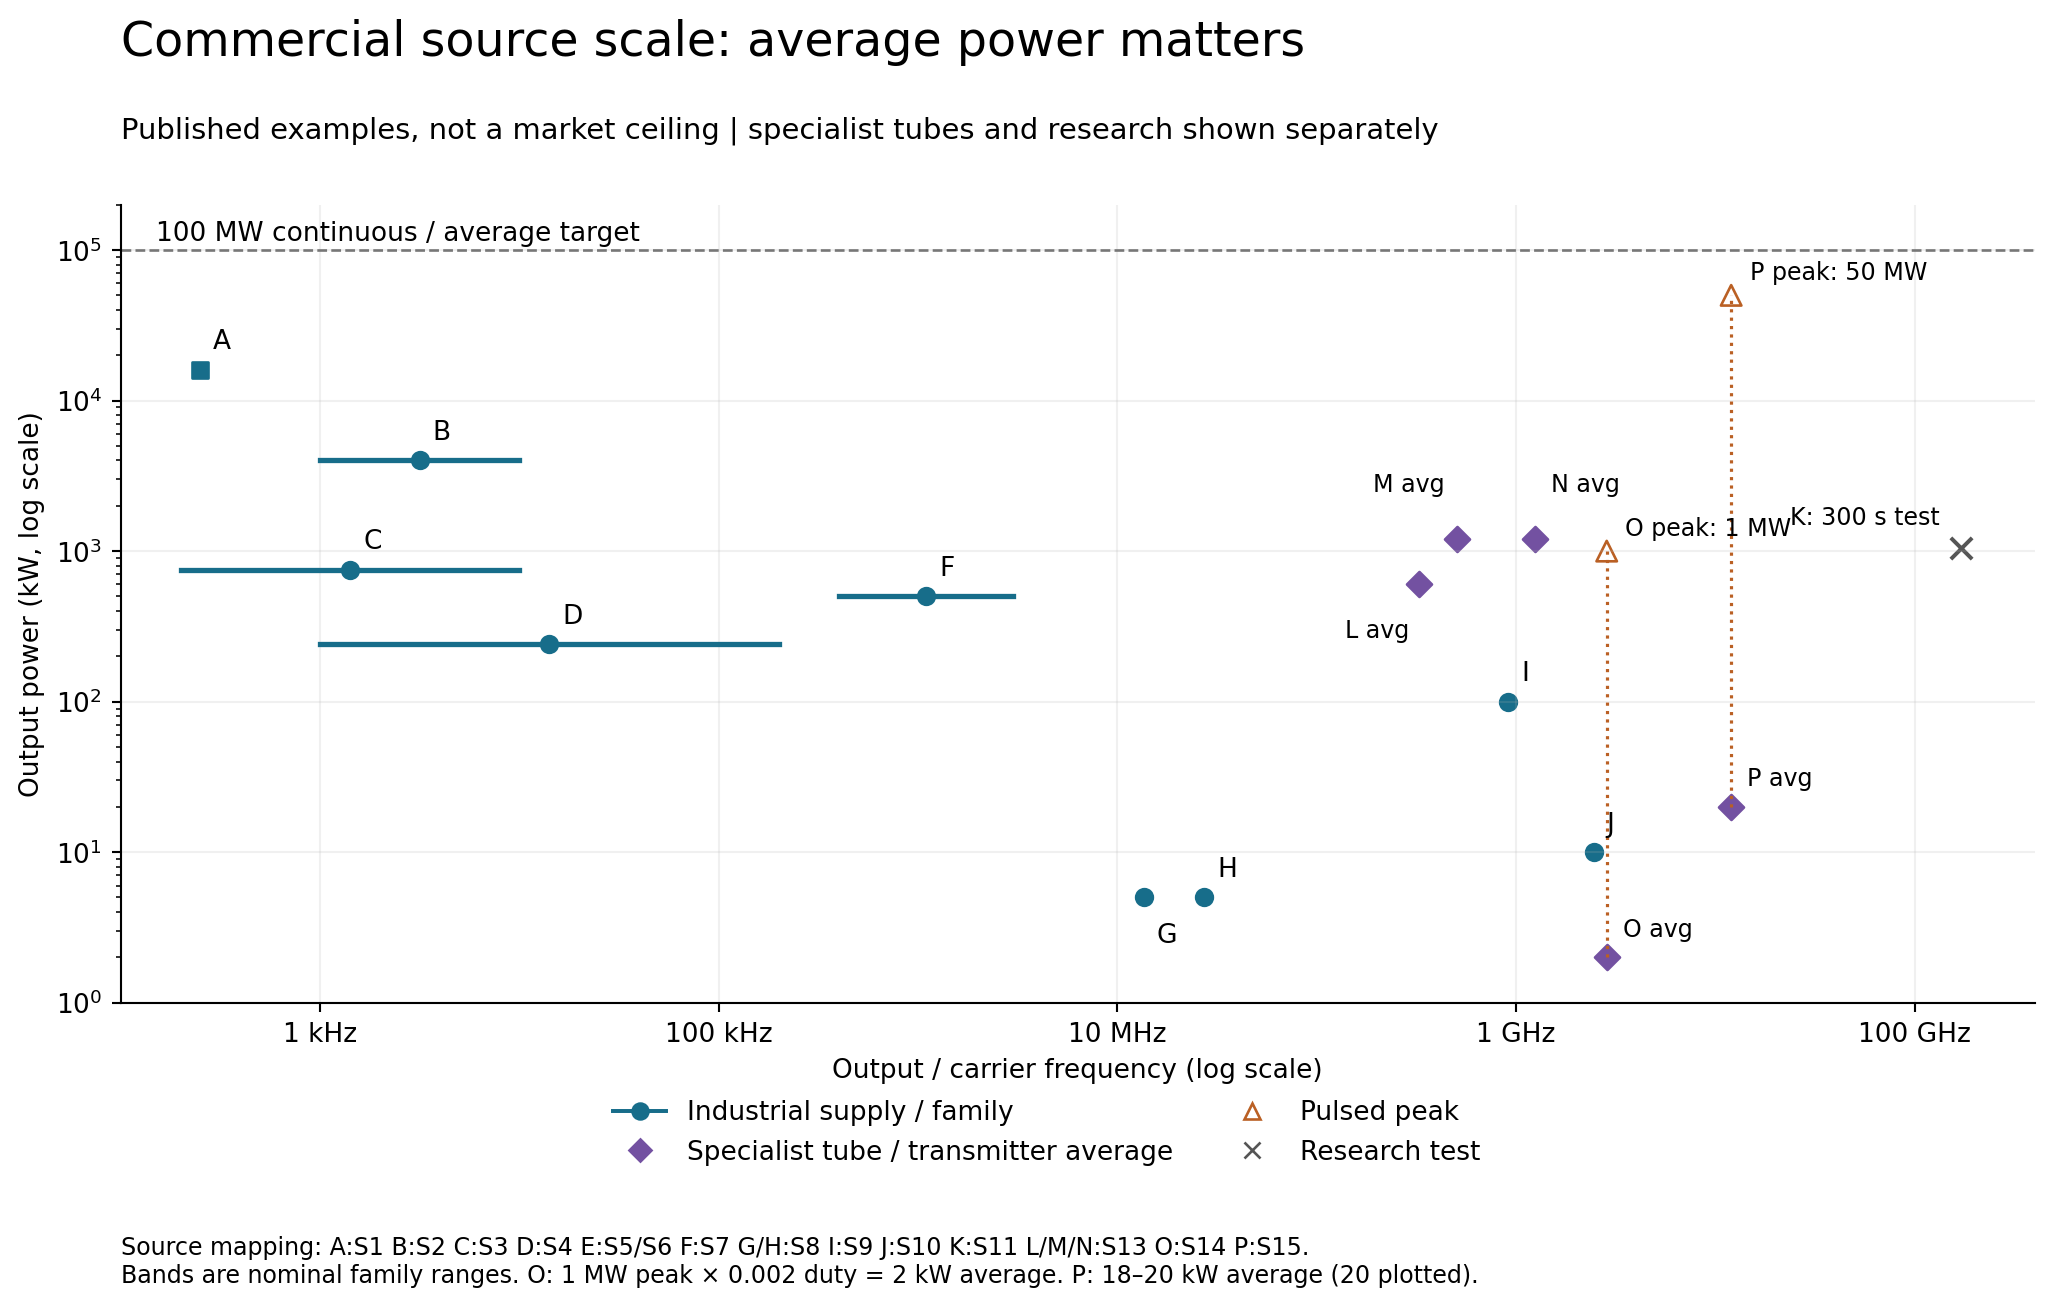
\includegraphics[width=.85\linewidth]{commercial_scale.png}
\caption{Scale of selected supplies and commercial specialist sources. Pulsed peaks are separated from average output; the 170~GHz gyrotron is a 300~s research test [S11]. This is an evidence map, not the maximum commercially attainable power at each frequency.}
\label{fig:scale}
\end{figure}

For rectangular pulses, $P_{\mathrm{avg}}=P_{\mathrm{peak}}\tau f_{\mathrm{rep}}$, where $\tau$ is pulse width and $f_{\mathrm{rep}}$ is repetition frequency, distinct from the RF carrier frequency. CPI reports 50~MW peak devices with only 18--20~kW average output [S15]. Pulsing may enable a different reaction trajectory, but the average heat demand remains. At 20~kW per source, 100~MW would require 5,000 sources arithmetically, before redundancy or delivery losses.

\begin{figure}[H]
\centering
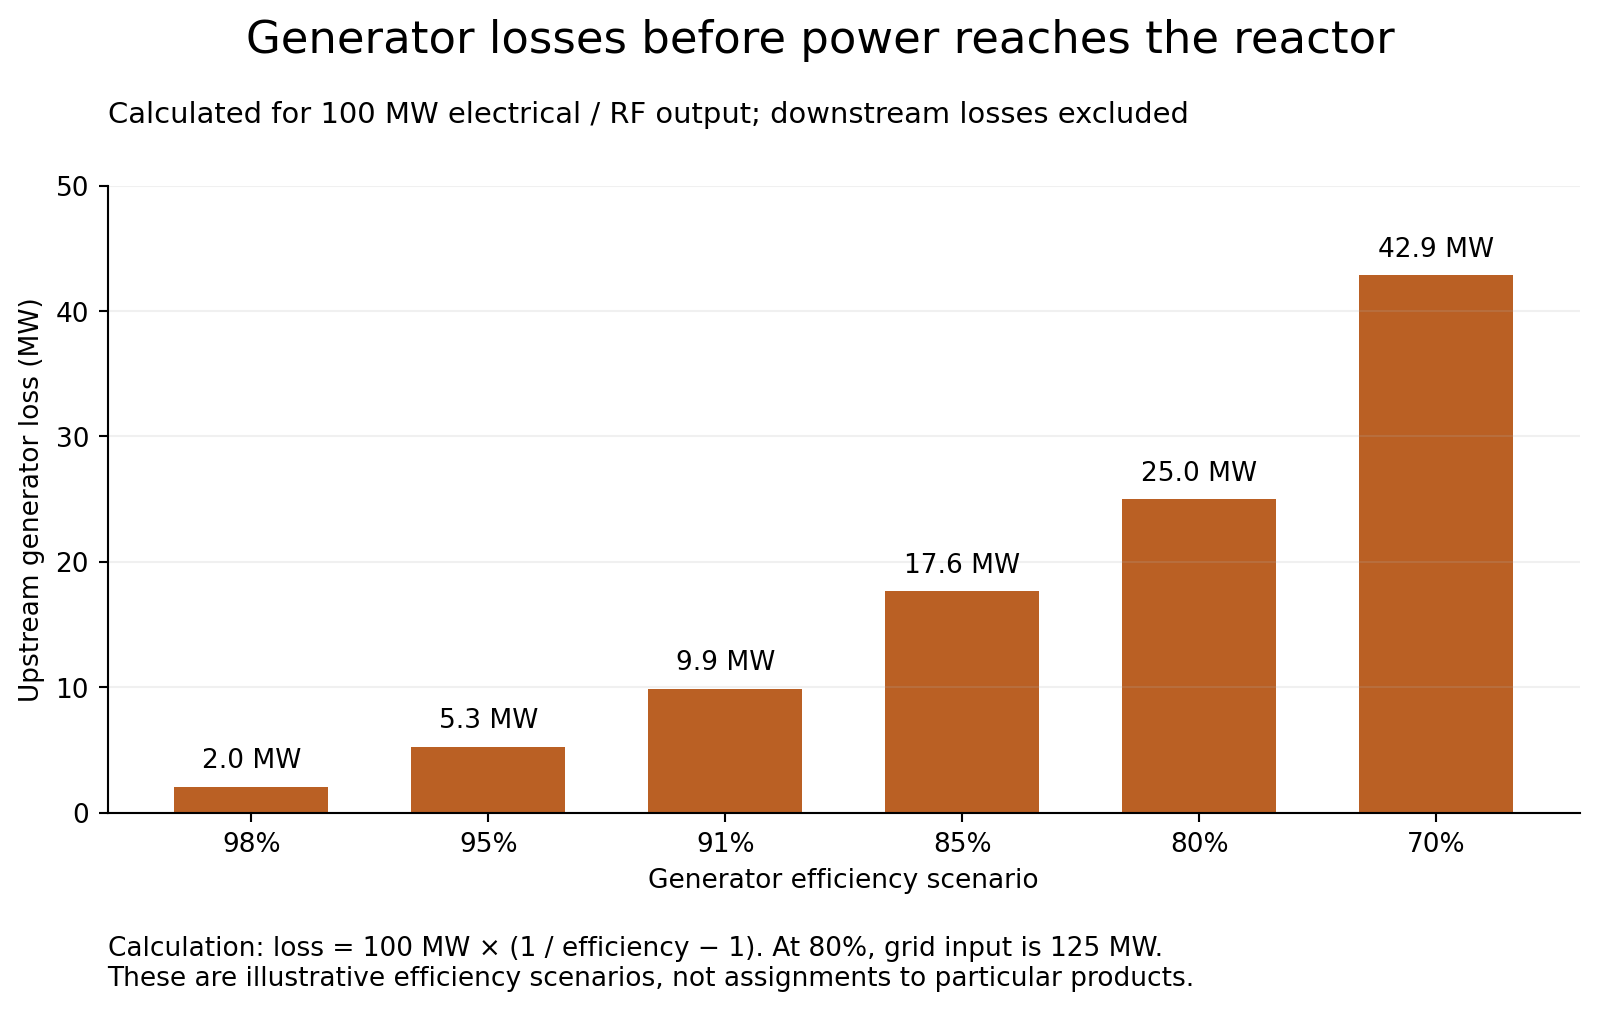
\includegraphics[width=.73\linewidth,height=.22\textheight,keepaspectratio]{upstream_losses_100mw.png}
\caption{Calculated upstream losses for 100~MW generator output: $P_{\mathrm{loss}}=100(1/\eta_{\mathrm{gen}}-1)$~MW. At 80\%, input is 125~MW and generator loss is 25~MW, before transmission, matching or reactor losses. Values are scenarios, not additional measurements.}
\label{fig:loss}
\end{figure}

\clearpage
\section{Reactor matching}
Usable power depends jointly on frequency, output voltage, current, complex load impedance and reactor geometry. Mains voltage, internal DC/beam voltage, generator output voltage and reactor electrode voltage must be distinguished. Matching networks transform voltage and current; at microwave frequencies, modal power and the spatial electric field are generally more informative than a geometry-independent terminal voltage.

For a linear sinusoidal load with admittance $Y=G+jB$, using RMS quantities,
\begin{equation}
P=V^2G,\qquad Q=-V^2B,\qquad I=V\sqrt{G^2+B^2}.
\end{equation}
An ideal capacitance absorbs no average power. Real dissipation must occur through conduction or dielectric losses in the intended region. For a homogeneous parallel-plate material, area $A$, gap $d$ and capacitance $C=\epsilon_0\epsilon_r'A/d$,
\begin{equation}
P=V^2\left[\frac{\sigma A}{d}+2\pi f C\tan\delta\right],
\label{eq:load}
\end{equation}
where $\tan\delta$ excludes the separately represented conduction loss to avoid double counting [S17]. For the purely dielectric example ($\sigma=0$), fixed $C$ and $\tan\delta$ give $V\propto f^{-1/2}$ at fixed power. Thus lower frequency may reduce conversion losses while increasing the required reactor voltage.

\begin{figure}[ht]
\centering
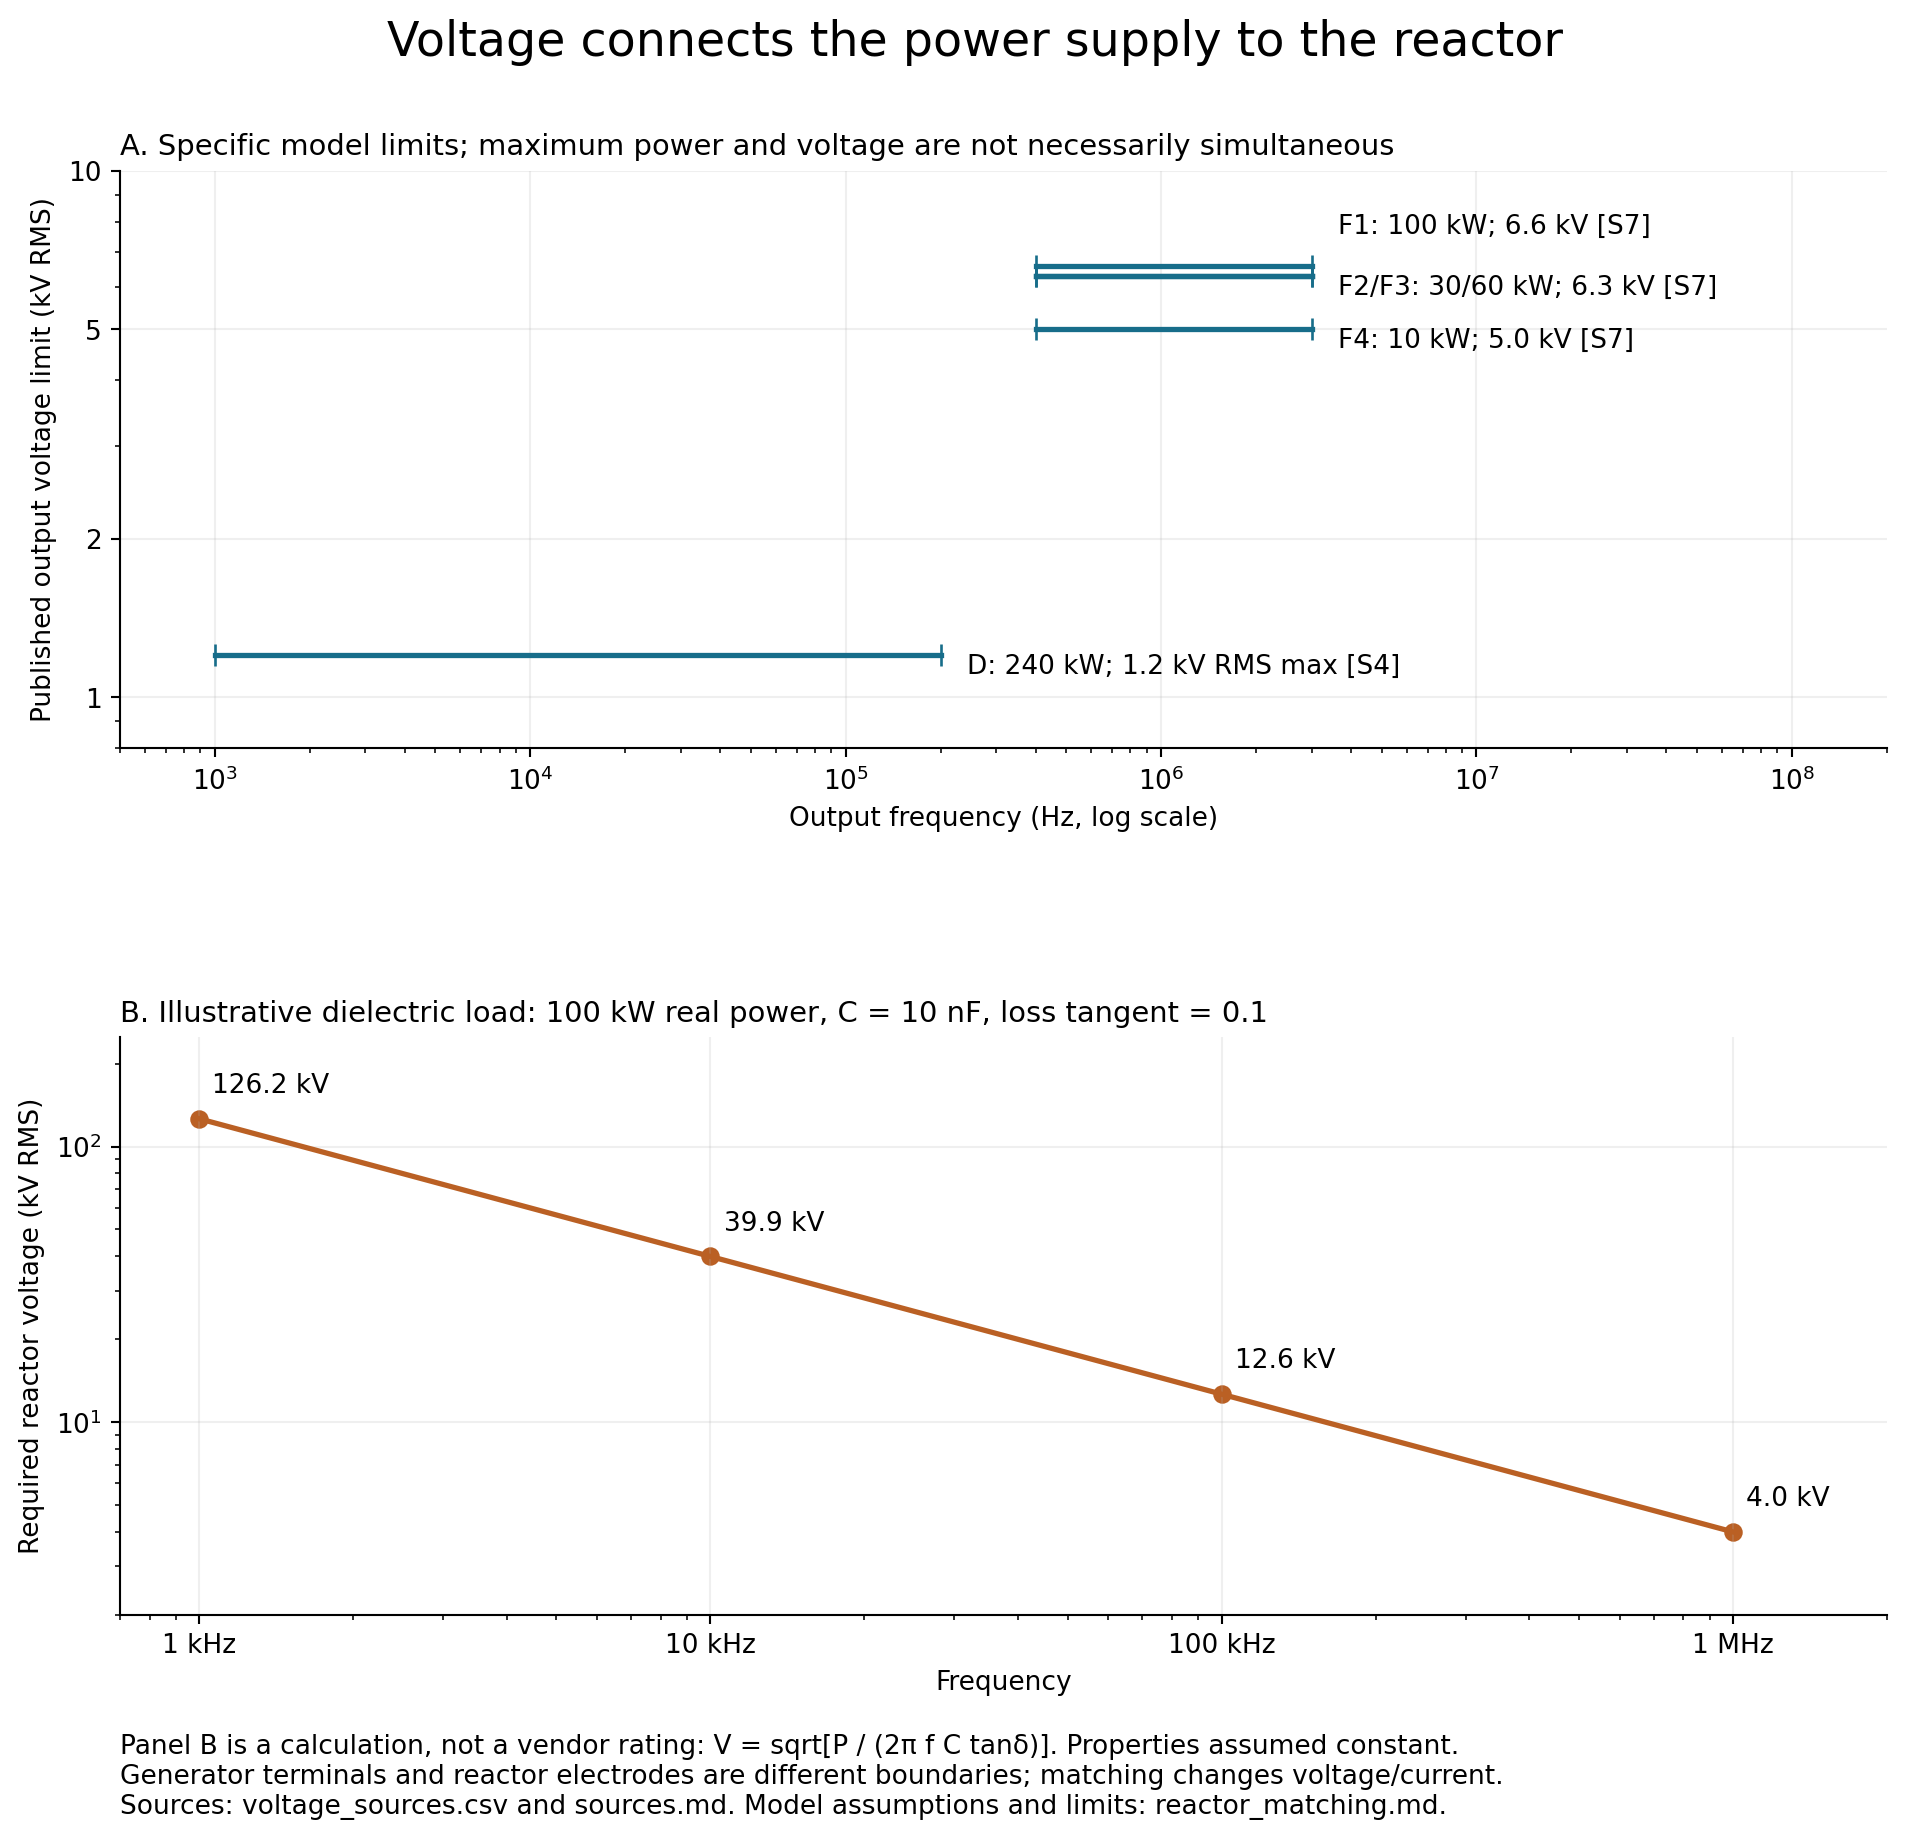
\includegraphics[width=\linewidth,height=.46\textheight,keepaspectratio]{voltage_and_reactor_matching.png}
\caption{Published model-specific output-voltage maxima [S4,S7] and a separate illustrative load calculation. The example is not a catalyst-bed prediction; material properties are assumed constant. Generator and reactor voltages need not coincide after matching.}
\label{fig:voltage}
\end{figure}

In the example, 100~kW real power with $C=10$~nF and $\tan\delta=0.1$ requires about 40~kV RMS at 10~kHz, versus 4~kV at 1~MHz. The reactive power magnitude is 1~MVAr in either case. Resonant compensation can reduce the generator's reactive demand, while large currents and voltages remain inside the matching circuit.

The next step is to measure complex impedance versus frequency, temperature and composition, and combine this with electrode geometry, insulation limits and average power per section. Frequency selection should minimise total electrical demand for the desired chemical output, subject to acceptable fields, currents, matching losses and deposition uniformity. A low-kilohertz design is a hypothesis to test against these constraints, not a conclusion established by converter efficiency alone.

\clearpage
\section*{Sources and reproducibility}
\small
The figures use public manufacturer claims and primary technical reports, not independently harmonised measurements. A listing does not confirm current delivery availability. Missing values remain missing; individual maxima are not assumed simultaneous. The source identifiers below match the figures and accompanying CSV files.

\begin{description}
\setlength{\itemsep}{2pt}
\item[S1] \href{https://abpinduction.com/wp-content/uploads/2020/02/ABP-Inductive_melting_in_steelworks_M._Chaabet_E._Doetsch.pdf}{ABP, \emph{Inductive melting in steelworks} (2015)}, PDF pp.~3,5. 16~MW/250~Hz supply and 126~MW aggregate installation.
\item[S2] \href{https://www.sms-elotherm.com/en/service/retrofit/converters}{SMS Elotherm, ELOMAT converters}. LLC family: 0.4--4~MW, 1--10~kHz.
\item[S3] \href{https://www.induction-furnaces.com/new-furnaces/pulsar-igbt-inverter-technology/}{Meltech, Pulsar IGBT}. 75--750~kW, 0.2--10~kHz; approximately 98\% operating efficiency.
\item[S4] \href{https://www.trumpf.com/en_US/products/power-electronics/generators-for-industrial-heating/truheat-mf/truheat-mf-serie-7000-g2/}{TRUMPF, TruHeat MF 7000 G2}. Model 7240: 240~kW, 1--200~kHz in model table, 91\%; maxima 1,200~V RMS and 1,120~A RMS.
\item[S5] \href{https://induction.ceia.net/en-IT/product/power-cube-sa-400-series}{CEIA, SA/400 family}. Quoted efficiency $>96\%$; measurement boundary requires confirmation.
\item[S6] \href{https://induction.ceia.net/es-EC/about-us/news/48}{CEIA, SA/400 announcement}. 100--400~kHz band and 50~kW version; see S16 for input/output distinction.
\item[S7] \href{https://www.trumpf.com/de_DE/produkte/leistungselektronik/generatoren-zur-industriellen-erwaermung/truheat-hf/truheat-hf-serie-7000/}{TRUMPF, TruHeat HF 7000}. Family headline up to 500~kW, 0.4--3~MHz. Specific 10--100~kW models have 5.0--6.6~kV RMS output maxima; these do not define the 500~kW model voltage.
\item[S8] \href{https://pct.comet.tech/en/products/synertia_rf_power_delivery_platform/synertia_rf_generator}{Comet, Synertia RF generators}. Selected 5~kW models at 13.56 and 27.12~MHz; family efficiency $>70\%$.
\item[S9] \href{https://www.microwavetechniques.com/industrial-microwave-generators/100-kw-mtx/}{Microwave Techniques, MTX100}. 100~kW at 915~MHz; generator operation approaching 80\% efficiency.
\item[S10] \href{https://www.sairem.com/wp-content/uploads/2021/01/SAIREM-MW-technology-guide-for-lab-grown-diamonds-applications.pdf}{SAIREM, microwave plasma guide}, printed p.~7. GMP100: 10~kW, 2,450~MHz, quoted power efficiency 85\%; boundary requires confirmation.
\item[S11] \href{https://conferences.iaea.org/event/214/contributions/17030/}{QST, ITER gyrotron performance tests, IAEA FEC (2021)}. 1.05~MW at 170~GHz, 50.6\% gyrotron efficiency, 300~s test; excludes full upstream plant losses.
\item[S12] \href{https://www.sairem.com/microwave-radiofrequency-equipment/industrial-generators/evomag-915-mhz-magnetron-generator/}{SAIREM, EvoMag 915}. 100~kW units, $>80\%$ efficiency and several-MW container combinations; contextual evidence, not a plotted point.
\item[S13] \href{https://etd.canon/en/product/category/microwave/klystron.html}{Canon, commercial klystron lineup}. E37705: 600~kW/325~MHz/60\%; E3732 and E3718: 1.2~MW at 508.6/508.9~MHz and 1,250~MHz respectively, 63\%. CW tube ratings, not complete generator efficiencies.
\item[S14] \href{https://www.cpi-edb.com/docs/datasheets/163/VPS3499%20KLYSTRON%20TRANS%20%20NF%20FINAL%2012-19-24.pdf}{CPI, VPS3499 transmitter datasheet (2024)}, p.~3. 2.7--3.0~GHz, 1~MW peak, RF duty 0.002; calculated average 2~kW. Figure plots band midpoint.
\item[S15] \href{https://indico.jlab.org/event/722/contributions/13920/}{CPI, \emph{Developments in High Efficiency Klystrons} (2024)}. XL4/XL5 class: 50~MW peak, 18--20~kW average, approximately 40\% tube efficiency. Representative 12~GHz point, not an exact specification of both models.
\item[S16] \href{https://induction.ceia.net/it-IO/product/power-cube-sa-400-series}{CEIA, detailed SA/400 specifications}. 50~kW is maximum input power; inductor kVAR rating is reactive power. Excluded from output-power comparison.
\item[S17] \href{https://doc.comsol.com/6.3/doc/com.comsol.help.acdc/acdc_ug_modeling.06.24.html}{COMSOL, Modeling losses in the frequency domain}. Conductivity and dielectric-loss formulation underlying Eq.~\ref{eq:load}.
\end{description}
\raggedright

\textbf{Reproducibility.} The plotting script is \texttt{plot\_power\_systems.py}. Inputs are\par
\texttt{power\_sources.csv}, \texttt{high\_frequency\_sources.csv} and \texttt{voltage\_sources.csv}. Detailed qualifications appear in \texttt{sources.md} and \texttt{reactor\_matching.md}. Compile this document from its directory with \texttt{pdflatex power\_systems\_report.tex} (twice to resolve references).
\end{document}
